\section{Data characteristics}
\label{sec:data_charcteristics}

This section describes datasets used for the experiments.
Additionally, statistics and error characteristics of datasets are discussed.

\subsection{Datasets}

\begin{table}[!t]
\caption{\label{tab:datasets_table}Datasets}
\centering
\begin{tabular}{r|K|K|K|K|H|K}
\toprule
 & \colCenter{\#rows} & \colCenter{\#cols} & \colCenter{Clean}  & \colCenter{Dirty}  & \colCenter{\#Cat} & \colCenterNoRight{\#Numeric}\\
\midrule
beers    &   2410 & 11 &  233 \textsc{KB} &  255 \textsc{KB} &  8 & 3 \\
flights  &   2376 &  7 &  173 \textsc{KB} &  155 \textsc{KB} &  7 & 0 \\
hospital &   1000 & 20 &  303 \textsc{KB} &  303 \textsc{KB} & 20 & 0 \\
movies   &   7390 & 17 & 4400 \textsc{KB} & 4600 \textsc{KB} & 14 & 3 \\
rayyan   &   1000 & 11 &  273 \textsc{KB} &  273 \textsc{KB} &  9 & 2 \\
tax      & 200000 & 15 & 14,6 \textsc{MB} & 14,6 \textsc{MB} & 10 & 5 \\
\bottomrule    
\end{tabular}
\end{table}


To evaluate the performance of the benchmark, six public datasets were used from \textcite{MahdaviAFMQST2019, MahdaviA2020} and available on GitHub~\footnote{\url{https://github.com/BigDaMa/raha/tree/master/datasets}}.
All datasets have a clean and dirty version.
In Table~\ref{tab:datasets_table} datasets and their main characteristics are presented.

\textbf{Beers} is a real-world dataset. It has been collected by web scraping, and was cleaned manually.
It is used in \textcite{MahdaviAFMQST2019, MahdaviA2020},
and the source can be be tracked to \textcite{Hould2017WEB, Hould2017KAGGLE}. 
The dataset contains information about different beer sorts, respective bottles and their producers.

\textbf{Flights} is a real-world dataset that originally was collected by \textcite{LiDLMS2015}. 
It is used in many projects \cite{holodetect, raha, LiDLMS2015}.
This dataset contains information on arrival and departure of flights.
The source of this dataset is \textcite{LiDLMS2015}.

\textbf{Hospital} data is taken from US Department of Health \& Human Services~\footnote{\url{http://www.hospitalcompare.hhs.gov} (Not working anymore)}. 
It is frequently used \cite{RestatGCS2022, ChuIP2013, DallachiesaEEEIOT2013, HeidariMIR2019,MahdaviAFMQST2019, MahdaviA2020, RekatsinasCIR2017}.
The dataset contains information about providers, their addresses, contacts and measurements they do.
In the experiments, a fraction of the whole dataset is used.
The fraction is published in GitHub~\footnote{\url{https://github.com/BigDaMa/raha/tree/master/datasets}}.

Both, \textit{flights} and \textit{hospital}, were obtained along with ground truth from \textcite{holodetect}.

\textbf{Movies} is a dataset that is available in the Magellan repository~\cite{DasDGGKGP2016, KondaDSDABLPZNPKDR2016}.
It was collected by web scraping Rotten Tomatoes~\footnote{\url{https://www.rottentomatoes.com/}} and IMBD~\footnote{\url{https://www.imdb.com/}}.
The data describes movies, their cast and ratings. 
Interestingly, one of the columns is \textsc{description} that is free text.

\textbf{Rayyan} is also a real-world dataset. 
It was cleaned by the owners~\cite{QuzzaniHFE2016} themselves, and is used in \textcite{MahdaviAFMQST2019, MahdaviA2020}.
The dataset summarizes articles, their characteristics such as publisher, volume, language etc.

\textbf{Tax} is a large synthetically created dataset from the BART~\cite{bart} repository.
It summarize information about tax payers and personal information that is important for the tax estimation.

\subsection{Data and error characteristics}
\label{sec:data_characteristics}
Main goals during data generation is to maintain error characteristics and  statistics of the original dirty dataset in the generated dirty dataset.
In this Section the characteristics of the original dirty input and the clean data is discussed and explained. 

\textbf{The main objective} is preservation of distinct values, min, max, mean, and distributions of typos, missing values, outliers, replacements and swaps.
These aggregate statistics are important because they contain information about every value.
For instance, mean shows presence of outliers or missing values.
Similarly, maintenance of frequencies of distinct values allows one to preserve error and data distribution while scaling up.

\textbf{The error distribution} of the different datasets is presented in Table~\ref{tab:dirty_num_errors}. 
Graphical representations of the errors include: The percentages of different error types in each dataset are shown in Figure~\ref{exp:errors_percent} and count - in Figure~\ref{exp:errors_count}.
In the \textit{beers} dataset only two types of errors are present: Typos and missing values. 
Interestingly, one column \textsc{ounces} was classified as fully missing because it was transferred from integer to string, e.g. \textsc{12} is turned into \textsc{12 oz} or \textsc{12 ounce}, and there are many missing values in the \textsc{ibu} column.
Then the \textit{flights} dataset contains the biggest count of typos over all  datasets. 
Most of them are in \textsc{sched\_dep\_time} column, e.g. \textsc{6:55 a.m.} is replaced by \textsc{12/02/2011 6:55 a.m.}.
The \textit{hospital} data has the smallest number of errors. 
Typos are in the \textsc{address\_1} column, while missing values are present in \textsc{address\_1}, \textsc{address\_2}, \textsc{address\_3}.
The \textit{movies} dataset contains the most text columns such as \textsc{name}, \textsc{description}, \textsc{director}, \textsc{creator}, \textsc{release\_date}, all of them contain typos. Additionally, in the column \textsc{rating\_count} $5737$ values are missing.
The \textit{tax} dataset contains all five error types. 
Together with typos, missing values and replacements, there are outliers, e.g. \textsc{salary} of \textsc{100000000}, and swaps between \textsc{f\_name} \& \textsc{l\_name}, \textsc{salary} \& \textsc{rate}, and \textsc{l\_name} \& \textsc{city}. 

\textbf{In general}, there are not many outliers detected.
First, the chosen datasets contain mostly text features what means that there are no outliers in the columns.
Second, for outlier detection only basic techniques such as IQR or by standard deviation were used. 
This means that contextual and collective outliers are not detected, but they are treated as different error type, because all differences between clean and dirty datasets are classified as faulty cells.
There are also not many swaps in the given data, although this is a common mistake in real-world datasets.

\begin{figure}[!t]
    \centering
    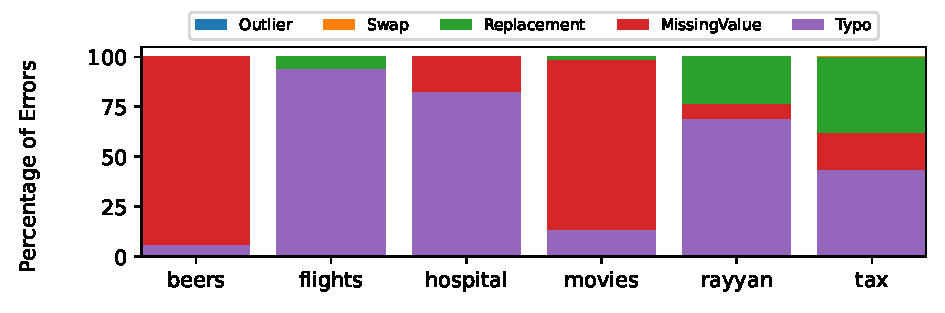
\includegraphics[width=\textwidth]{figures/plot/error_percent/errors_percent.pdf}
    \caption{Percentage of errors}
    \label{exp:errors_percent}
\end{figure}

\begin{figure}[!t]
    \centering
    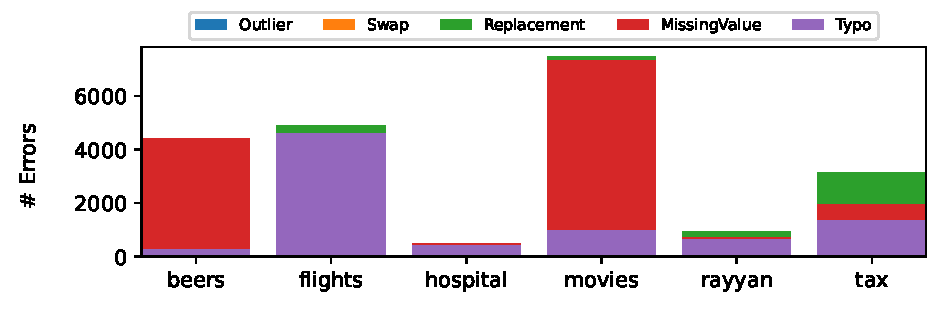
\includegraphics[width=\textwidth]{figures/plot/error_percent/errors.pdf}
    \caption{Frequency of errors}
    \label{exp:errors_count}
\end{figure}

\begin{table}[!t]
\centering
\caption{\label{tab:dirty_num_errors}Dirty dataset error characteristics}
\begin{tabular}{r|K|K|K|K|K}
\toprule
                     & \colCenter{Outliers} & \colCenter{Typos} & \colCenter{MV}             & \colCenter{Rep}              & \colCenterNoRight{Swaps}   \\ \midrule
beers                & 0        & 254   & 4170           & 0                & 0       \\
flights              & 0        & 4606  & 0              & 314              & 0       \\
hospital             & 0        & 417   & 92             & 0                & 0       \\
movies               & 0        & 982   & 6346           & 141              & 0       \\
rayyan               & 0        & 649   & 75             & 224              & 0       \\
tax                  & 2        & 1367  & 588            & 1200             & 4       \\ \bottomrule
\end{tabular}
\end{table}

\textbf{Distinct values} are also interesting in terms of data distribution, and impact of errors on number of distinct items.
Figure~\ref{exp:distinct_values_datasets} shows how the distinct value set in columns changes after error introduction. 
The x-axis represents each feature of the dataset, while y-axis is log-scaled and shows number of distinct values. 
Blue color represents clean data, red color - dirty.
It is noticeable that in \textit{bears}, as stated earlier, one column is treated as completely missing.
On the other hand, in \textit{hospitals} and \textit{flights} the number of distinct item increases.
This happens because of a high amount of typos in both datasets.

\begin{figure}[!t]
    \centering 
    \centering
\begin{subfigure}{0.32\textwidth}
    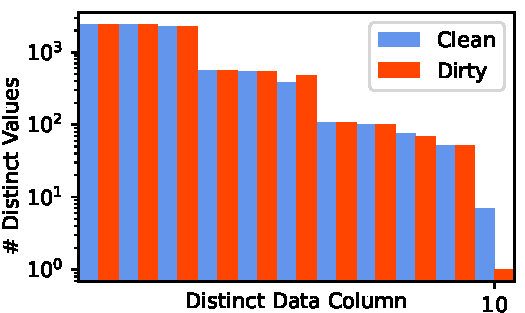
\includegraphics[width=\textwidth]{figures/plot/distinct/beers_distinct/combined.pdf}
    \caption{\label{exp:d1}Bears}
    \label{exp:distincts_bears}
\end{subfigure}
\hfill
\begin{subfigure}{0.32\textwidth}
    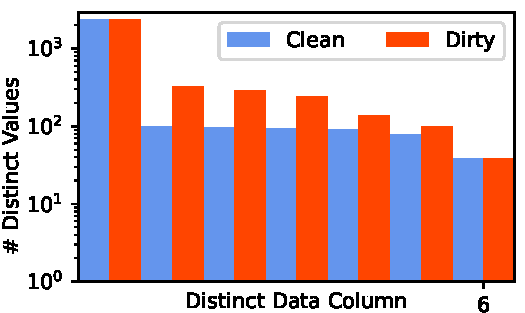
\includegraphics[width=\textwidth]{figures/plot/distinct/flights_distinct/combined.pdf}
    \caption{Flights}
    \label{exp:distincts_flights}
\end{subfigure}
\hfill
\begin{subfigure}{0.32\textwidth}
    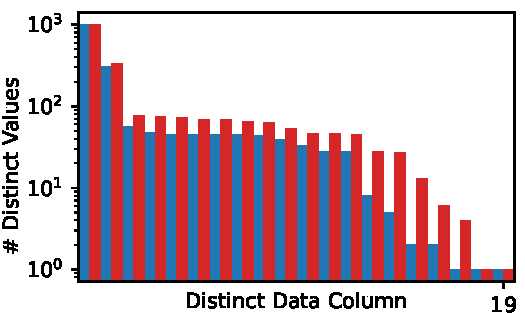
\includegraphics[width=\textwidth]{figures/plot/distinct/hospital_distinct/combined.pdf}
    \caption{Hospital}
    \label{fig:distincts_hospitals}
\end{subfigure}
\hfill
\begin{subfigure}{0.32\textwidth}
    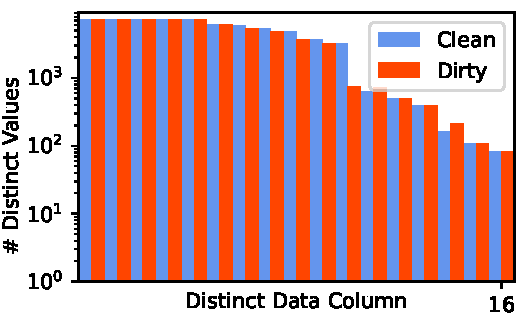
\includegraphics[width=\textwidth]{figures/plot/distinct/movies_distinct/combined.pdf}
    \caption{Movies}
    \label{exp:distincts_movies}
\end{subfigure}
\hfill
\begin{subfigure}{0.32\textwidth}
    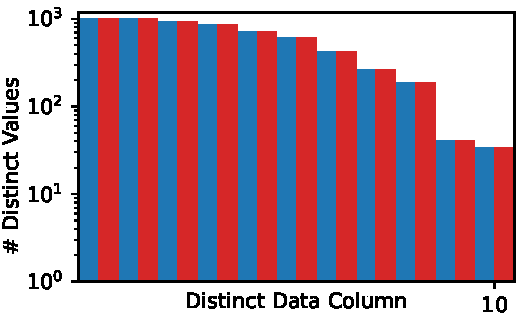
\includegraphics[width=\textwidth]{figures/plot/distinct/rayyan_distinct/combined.pdf}
    \caption{Rayyan}
    \label{exp:distincts_rayyan}
\end{subfigure}
\hfill
\begin{subfigure}{0.32\textwidth}
    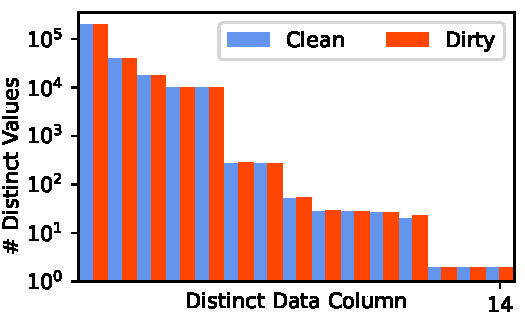
\includegraphics[width=\textwidth]{figures/plot/distinct/tax_distinct/combined.pdf}
    \caption{Tax}
    \label{exp:distincts_tax}
\end{subfigure}
\hfill
\caption{Distinct values distribution of clean and dirty datasets}
\label{exp:distinct_values_datasets}
\end{figure}

\textbf{Scaling the datsets} effect the error distribution, and is shown for tax in Table~\ref{tab:local_errors_tax} and for the other datasets in Appendix~\ref{apendix:error_counts_scaling}.
% TODO Describe

\begin{table}[!t]
\caption{\label{tab:local_errors_tax} Local error distribution in tax}
\centering
\begin{tabular}{r|K|K|K|K|K}
\toprule
\colCenter{Scale} & \colCenter{Outliers} & \colCenter{Typos} & \colCenter{MV} & \colCenter{Rep} & \colCenterNoRight{Swaps}  \\ \midrule
 1  &   2 &   1367 &    588 &    1200 &    4 \\
 2  &   4 &   2734 &   1176 &    2400 &    6 \\
 4  &   8 &   5468 &   2352 &    4800 &   12 \\
 8  &  16 &  10936 &   4704 &    9600 &   23 \\
16  &  32 &  21842 &   9408 &   19200 &   48 \\
32  &  64 &  43744 &  18816 &   38400 &   96 \\
64  & 128 &  87488 &  37632 &   76800 &  189 \\
128 & 256 & 174976 &  75264 &  153600 &  378 \\
256 & 512 & 349952 & 150528 &  307200 &  756 \\
\bottomrule
\end{tabular}
\end{table}

\textbf{Scaling distinct values} is more interesting, and is shown for tax in Table~\ref{tab:dist_errors_tax} and the other datasets in Appendix~\ref{apendix:distinct_errors_scaling}.
% TODO Describe

\newcolumntype{S}{>{\raggedleft\arraybackslash$}p{2.0cm}<{$}}

\begin{table}[!t]
\caption{\label{tab:dist_errors_tax} Local errors distincts in tax}
\centering
\begin{tabular}{r|H|H|H|H|K|K|S}
               & \multicolumn{2}{c|}{\textbf{Typos}}   & \multicolumn{2}{c|}{\textbf{MV}} & \multicolumn{2}{c|}{\textbf{Distinct}}  & \multicolumn{1}{c}{\textbf{Outliers}}\\
\colCenter{Scale} & \colCenter{Est} & \colCenter{Act} &  \colCenter{Est} & \colCenter{Act} & \colCenter{Est} & \colCenter{Act}   & \colCenterNoRight{Act}   \\ \midrule
1              & 81  & 81    & 6    & 6   & 275201   & 275201 &  2    \\
2              & 83  & 83    & 9    & 11  & 275260   & 275257 &  4    \\
4              & 84  & 84    & 15   & 16  & 275271   & 275261 &  4    \\
8              & 86  & 86    & 27   & 22  & 275293   & 275272 &  5    \\
16             & 89  & 89    & 51   & 28  & 275336   & 275286 &  5    \\
32             & 96  & 96    & 89   & 29  & 275413   & 275296 &  8    \\
64             & 107 & 107   & 138  & 23  & 275537   & 275306 &  12   \\ 
128            & 129 & 129   & 264  & 22  & 275813   & 275332 &  32   \\
\bottomrule
\end{tabular}
\end{table}

